\documentclass[a4paper,12pt]{article}
\usepackage[utf8]{inputenc}
\usepackage[T1]{fontenc}
\usepackage{graphicx}
\usepackage{enumitem}
\usepackage{geometry}
\usepackage{titling}
\usepackage{parskip}
\usepackage[colorlinks=true, allcolors=blue]{hyperref}
\usepackage{array}
\usepackage{booktabs}
\usepackage{listings}
\usepackage{array}
\usepackage{fancyvrb}
\usepackage[table]{xcolor}
\usepackage{hyperref}
\geometry{margin=2.5cm}

\lstset{
    backgroundcolor=\color{gray!10},
    basicstyle=\ttfamily\small,
    breaklines=true,
    frame=single,
    language=Python
}

\title{Práctica 3: Primeros módulos Odoo}
\author{Andrea Sofía Pais Dos Santos}
\date{\today}

\begin{document}
\setlength{\droptitle}{0.4\textheight} 
\maketitle
\thispagestyle{empty}
\newpage 


\vspace{7cm}

\section{Índice}

\begin{enumerate}[start=2]
    \item Introducción  .................................................................. página 3
    \item Implementación de módulo básico ................................. página 4
    \begin{itemize}
    \item Instalación del módulo "hola mundo"
    \end{itemize}
    \item Implementación del primer módulo ................................ página 5
    \begin{itemize}
    \item Instalación del módulo "lista de tareas"
    \item Problemas encontrados y soluciones
    \end{itemize}
    \item Modificación del primer módulo ..................................... página 10
    \begin{itemize}
    \item Modificación del módulo "lista de tareas"
    \end{itemize}
    \item Conclusiones ................................................................... página 12
\end{enumerate}
\newpage


\section{Introducción}

El objetivo de la práctica es mediante la creación y la implementación de módulos básicos, familiarizarse con el entorno de desarrollo de Odoo. Primero lo que
vamos a tener que hacer es activar el Modo Desarrollador, para ellos accedemos al enlace \href{https://www.odoo.com/documentation/17.0/es/applications/general/developer_mode.html}{Cambio a modo desarrollador}.

\vspace{0.5cm}
Para activar el modo desarrollador, nos situamos en "Ajustes Generales", bajamos hasta encontrar "Herramientras de desarrollador" y activamos la primera opción.

\vspace{0.5cm}
\begin{center}
    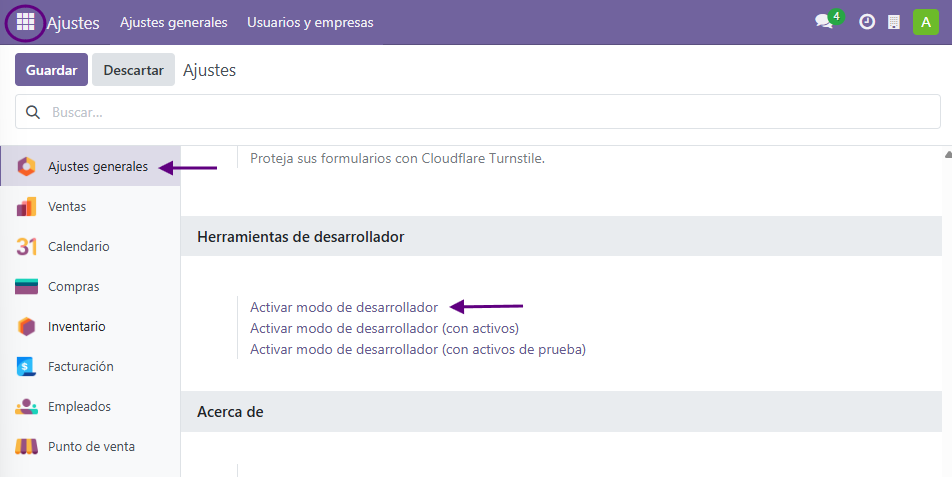
\includegraphics[height=8cm]{images/captura1.png}
\end{center}

\vspace{0.5cm}
Al activar el modo desarrollo nos aparece un icono de un "insecto" con un submenú que contiene herramientas para entender o editar información técnica.

\vspace{0.5cm}
\begin{center}
    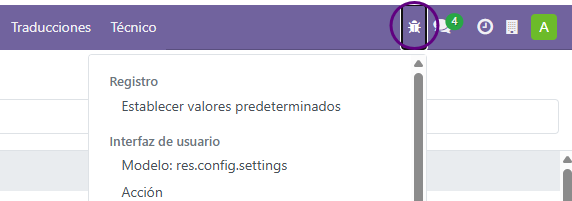
\includegraphics[height=4cm]{images/captura2.png}
\end{center}



\vspace{1cm}
\section{Implementación de módulo básico}

\subsection{Instalación del módulo "Hola mundo"}

\vspace{0.5cm}
\begin{itemize}
    \item Creamos una caperta para el módulo "hola mundo" en la carpeta addons. 
        \begin{lstlisting}[language=bash]
        mkdir addons/hola_mundo
        \end{lstlisting}
    \item Creamos los archivos vacíos siguientes:
        \begin{lstlisting}[language=bash]
        __init__.py
        __manifest__.py
        \end{lstlisting}
    \begin{center}
    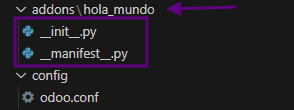
\includegraphics[height=3cm]{images/captura5.png}
    \end{center}
    \item Al ser un módulo sencillo en primer arcivo "init" puede estar vacío, mientras que al archivo
    "manifest" le vamos a añadir el siguiente ejemplo:
    \begin{Verbatim}[frame=single, fontsize=\small]
    {
        'name': 'Hola Mundo',
        'summary': 'Mi primer módulo Odoo',
        'description': 'Módulo básico de prueba para la práctica 3',
        'author': 'Andrea Sofía Pais Dos Santos',
        'version': '1.0',
        'depends': ['base'],
        'application': True,
        'category': 'Tools',
    }
    \end{Verbatim}
    \item En el entorno de desarrollo actualizamos la "lista de aplicaciones", buscamos el módulo "hola mundo".
    \vspace{0.5cm}
    \begin{center}
        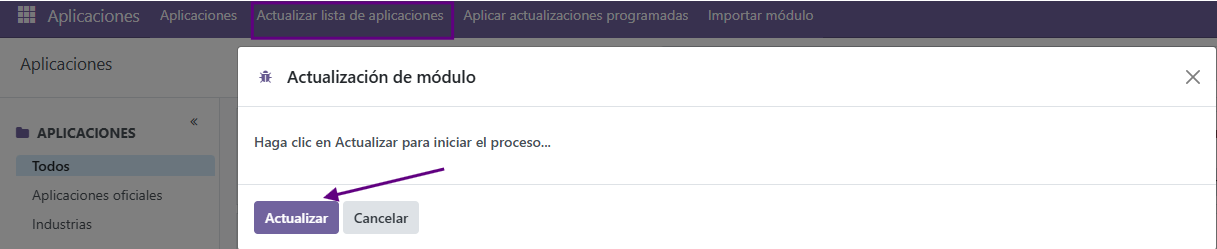
\includegraphics[height=3cm]{images/captura6.png}
    \end{center}
    \item Si haciendo lo anterior sigue sin salir el módulo, ejecutamos y volvemos a actualizar la lista de aplicaciones.
    \vspace{0.5cm}    
        \begin{lstlisting}[language=bash]
            docker-compose restart web
        \end{lstlisting}
    \item Buscamos el módulo "Hola Mundo" y lo activamos.
    \begin{center}
        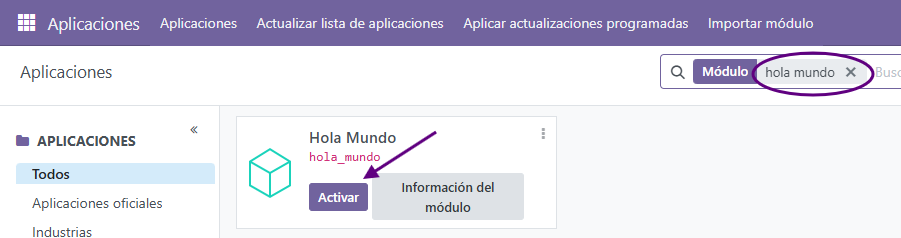
\includegraphics[height=3.5cm]{images/captura7.png}
    \end{center}
    \vspace{0.5cm} 
    \item En aplicaciones instaladas encontraremos el módulo "Hola mundo" con su respectiva información. 
    \vspace{0.5cm}
    \begin{center}
        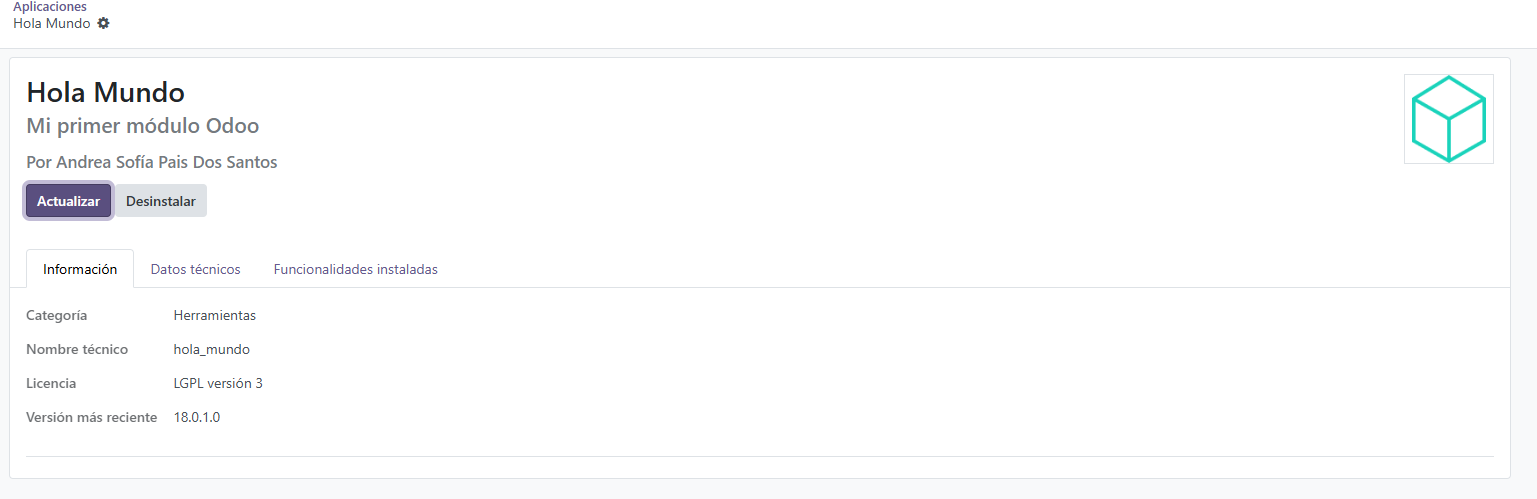
\includegraphics[height=5cm]{images/captura8.png}
    \end{center}
\end{itemize}


\vspace{1cm}
\section{Implementación del primer módulo}
\subsection{Instalación del módulo "lista de tareas"}
\begin{itemize}
    \item Creamos una carpeta para el módulo "lista de tareas"
    \begin{lstlisting}[language=bash]
        mkdir addons/lista_tareas
    \end{lstlisting}
    \item Para ayudarnos a crear el primer módulo vamos a usar la siguiente guía: \href{https://www.odoo.com/documentation/14.0/es/administration/odoo_sh/getting_started/first_module.html}{Primer módulo}, en el que vamos a usar "una plantilla de estructura de módulo" para realizarlo manualmente en mi caso.
    
    
\includegraphics[height=1cm]{images/captura12.png}

    \item Al descargar la plantilla en la carpeta que creamos nos genera la siguiente estructura de carpetas y archivos que modificaremos con la información que nos interese.
    \begin{center}
    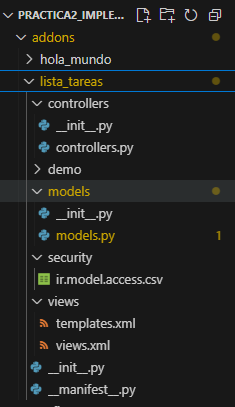
\includegraphics[height=7cm]{images/captura9.png}
    \end{center}
\end{itemize}
    Ahora vamos a rellenar los archivos con el código necesario para crear el módulo.

\begin{itemize}
    \item Vamos a empezar con los archivos "init", el primero \url{"addons/lista_tareas/__init__.py"}, le podemos estas importaciones:
    \begin{lstlisting}[language=Python]
        from . import controllers
        from . import models
    \end{lstlisting}
    \item Para el archivo \url{"addons/lista_tareas/models/__init__.py"} lo tenemos que rellenar con lo siguiente:
    \begin{lstlisting}[language=Python]
        from . import models
    \end{lstlisting}
    \item Para el archivo \url{"addons/lista_tareas/controllers/__init__.py"} le añadimos esto:
    \begin{lstlisting}[language=Python]
        from . import controllers
    \end{lstlisting}
    \item Ahora vamos con los archivos que tienen más contenido, empezamos con el archivo \url{"addons/lista_tareas/__manifest__.py"} le añadimos estos datos:
    \begin{Verbatim}[frame=single, fontsize=\small]
    # -*- coding: utf-8 -*-
    {
        'name': "Lista de tareas",
        'summary': """Sencilla Lista de tareas""",
        'description': """Sencilla lista para crear nuevo módulo""",
        'author': "Andrea Sofía Pais Dos Santos",
        'application': True,
        'category': 'Productivity',
        'version': '0.1',
        'depends': ['base'],
        'data': [
            'security/ir.model.access.csv',
            'views/views.xml',
        ],
    }
    \end{Verbatim}
        \item Ahora dentro del archivo \url{"addons/lista_tareas/controllers/controllers.py"} es un archivo que puede quedar vacío como en este caso.
        \item Dentro del archivo \url{"addons/lista_tareas/demo/demo.xml"} es un archivo que puede quedar vacío como en este caso.
        \item Ahora dentro del archivo \url{"addons/lista_tareas/models/models.py"} tenemos que añadir:
        \begin{Verbatim}[frame=single, fontsize=\small]
    from odoo import models, fields, api
    #Definimos el modelo de datos
    class lista_tareas(models.Model):
        #Nombre y descripcion del modelo de datos
        _name = 'lista_tareas.lista_tareas'
        _description = 'lista_tareas.lista_tareas'
        #Elementos de cada fila del modelo de datos
        #Los tipos de datos a usar en el ORM son
        tarea = fields.Char(string="Tarea")
        prioridad = fields.Integer(string="Prioridad")
        urgente = fields.Boolean(compute="_value_urgente", store=True)
        realizada = fields.Boolean(string="Realizada")
        @api.depends('prioridad')
        def _value_urgente(self):
            #Para cada registro
            for record in self:
                #Si la prioridad es mayor que 10, se considera 
                urgente, en otro caso no lo es
                if record.prioridad>10:
                    record.urgente = True
                else:
                    record.urgente = False
    \end{Verbatim}
    \item Ahora dentro del archivo \url{"addons/lista_tareas/security/ir.model.access.csv"} tenemos que añadir:
        \begin{Verbatim}[frame=single, fontsize=\small]
    id,name,model_id:id,group_id:id,perm_read,perm_write,perm_create,
    perm_unlink
    access_lista_tareas_user,lista.tareas.user,
    model_lista_tareas_lista_tareas,base.group_user,1,1,1,1
    \end{Verbatim}
    \item Ahora dentro del archivo \url{"addons/lista_tareas/views/view.xml"} tenemos que añadir:
        \begin{Verbatim}[frame=single, fontsize=\small]
    <odoo>
  <data>
  <!-- explicit list view definition -->
  <!-- Definimos como es la vista explicita de la litas-->
    <record model="ir.ui.view" id="lista_tareas.list">
      <field name="name">lista_tareas list</field>
      <field name="model">lista_tareas.lista_tareas</field>
      <field name="arch" type="xml">
        <list>
          <field name="tarea"/>
          <field name="prioridad"/>
          <field name="urgente"/>
          <field name="realizada"/>
        </list>
      </field>
    </record>
    <!-- actions opening views on models -->
    <!-- Acciones al abrir las vistas en los modelos-->
    <record model="ir.actions.act_window" id="lista_tareas.action_window">
      <field name="name">Listado de tareas pendientes</field>
      <field name="res_model">lista_tareas.lista_tareas</field>
      <field name="view_mode">list,form</field>
    </record>
    <!-- Top menu item -->
    <menuitem name="Listado de tareas" id="lista_tareas.menu_root"/>
    <!-- menu categories -->
    <menuitem name="Opciones Lista Tareas" id="lista_tareas.menu_1" 
    parent="lista_tareas.menu_root"/>
    <!-- actions -->
    <menuitem name="Mostrar lista" id="lista_tareas.menu_1_list" 
    parent="lista_tareas.menu_1" action="lista_tareas.action_window"/>
  </data>
</odoo>
    \end{Verbatim}
    
    \item Después de tener todos los archivos vamos a resetear, ejecutando lo siguiente:
    \begin{lstlisting}[language=bash]
        docker-compose restart web
    \end{lstlisting}
    \item Actualizamos la lista de aplicaciones como hicimos ateriormente y buscamos el módulo "lista de tareas" creado:

    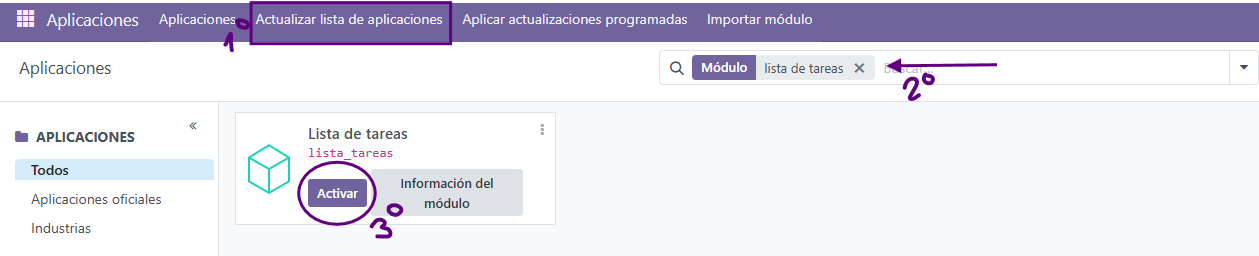
\includegraphics[height=3cm]{images/captura10.png}
\end{itemize}


\vspace{0.5cm}
\subsection{Problemas encontrados y soluciones}
Al activar el módulo de "lista de tareas" me sale un error que no me permite activar el módulo, investigué y parece ser que había que cambiar "tree" (formaba parte de la terminología antigua) por "list" (terminología nueva). "Tree" era para Odoo 16, ahora para Odoo 18 se usa "List".

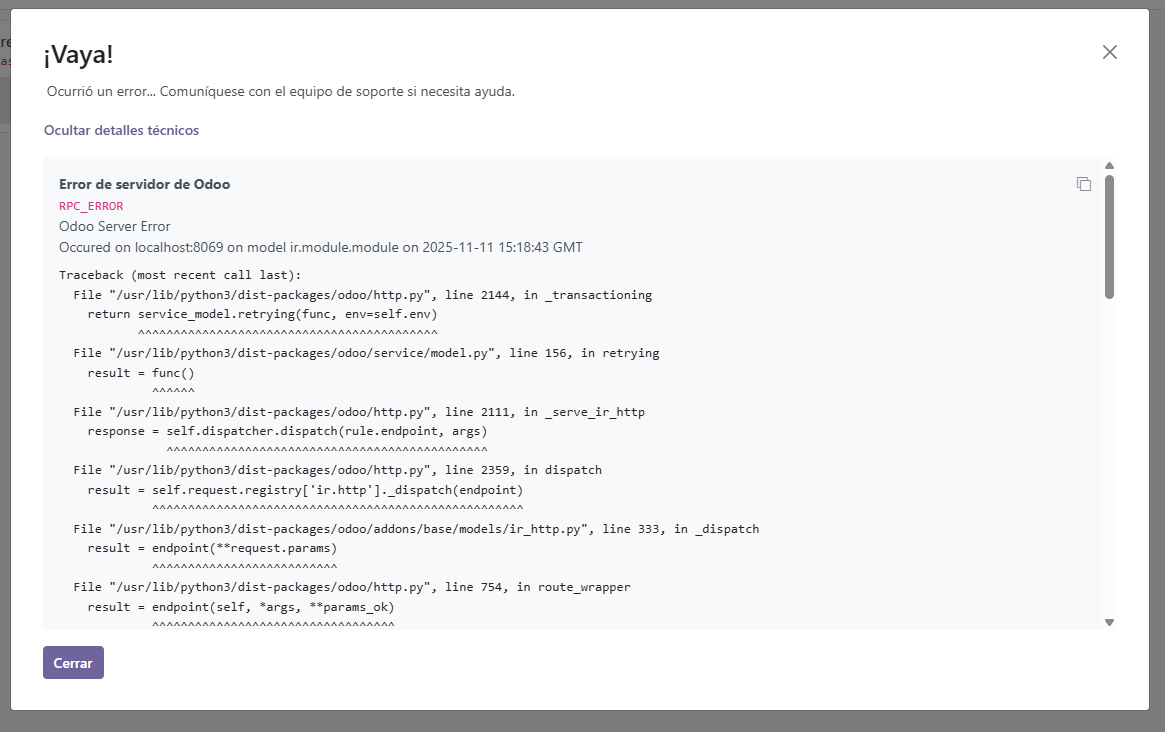
\includegraphics[height=10cm]{images/captura11.png}

\vspace{0.5cm}
Ya al cambiar eso me permite activar el módulo "lista de tareas". Ahora ya podemos crear nuestras tareas, aquí una de ejemplo: 

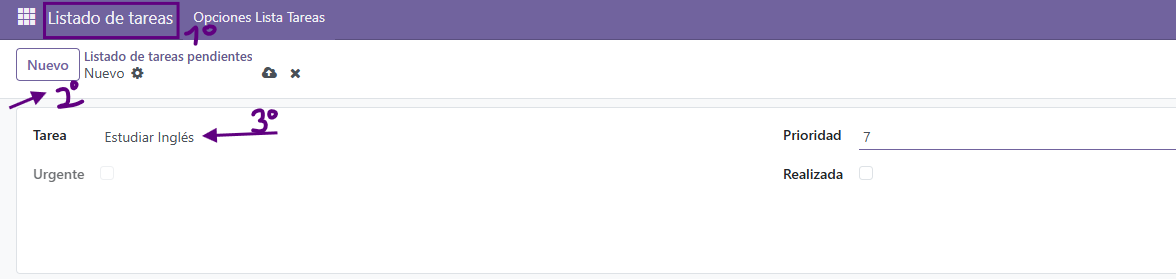
\includegraphics[height=4cm]{images/captura13.png}

\vspace{0.5cm}
Se pueden modificar en cualquier momento, añadir más, borrarlas, etc.

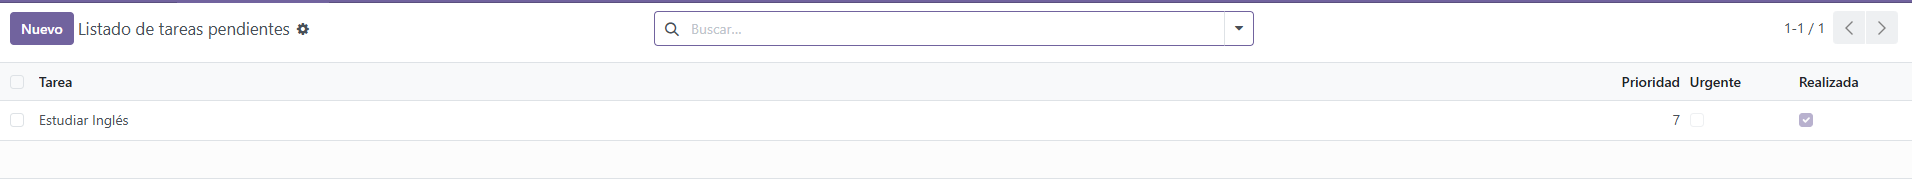
\includegraphics[height=1.6cm]{images/captura14.png}


\vspace{2cm}
\section{Modificación del primer módulo}

\subsection{Modificación del módulo "lista de tareas"}

Para este módulo como modificación extra se decidió agregar un apartado de un listado de categorías para clasificar las tareas y darle un poco más de estética a la interfaz al crear una nueva tarea.

Primero modificamos los archivos, en este caso tenemos que modificar: \url{addons/lista_tareas/models/models.py} y \url{addons/lista_tareas/views/views.xml}. En el primero vamos a añadir las categorías que nos interesa: 

\begin{Verbatim}[frame=single, fontsize=\small]
    categoria = fields.Selection([
        ("estudio","Estudio"),
        ("trabajo","Trabajo"),
        ("ocio","Ocio"),
        ("citas","Citas")
    ],string="Categoría",default="cita")
\end{Verbatim}

Hemos añadido el nombre de las categorñias que nos interesa y establecemos por defecto la categoría citas (por ejemplo para médico, entrevistas, eventos, etc).

Luego tenemos que añadir una modificación de la vista añadiendo la nueva funcionalidad que acabamos de crear:

\begin{Verbatim}[frame=single, fontsize=\small]
    <record model="ir.ui.view" id="lista_tareas_form">
      <field name="name">lista_tareas_form</field>
      <field name="model">lista_tareas.lista_tareas</field>
      <field name="arch" type="xml">
        <form>
          <sheet>
            <group>
            <!-- va a ser el título de este grupo -->
              <group string="La información principal">
                <field name="tarea" required="1"/>
                <field name="categoria"/>
                <field name="prioridad"/>
              </group>
              <!-- va a ser el título de este grupo -->
              <group string="Estado">
                <field name="realizada"/>
                <field name="urgente" readonly="1"/>
              </group>
            </group>
          </sheet>
        </form>
      </field>
    </record>
\end{Verbatim}

\vspace{2cm}
Luego de tener el código ya cambiado, nos vamos al entorno Odoo y volvemos a actualizar la lista de aplicaciones. Buscamos el módulo ya instalado "lista de tareas" y lo actualizamos.

\vspace{0.5cm}
\begin{center}
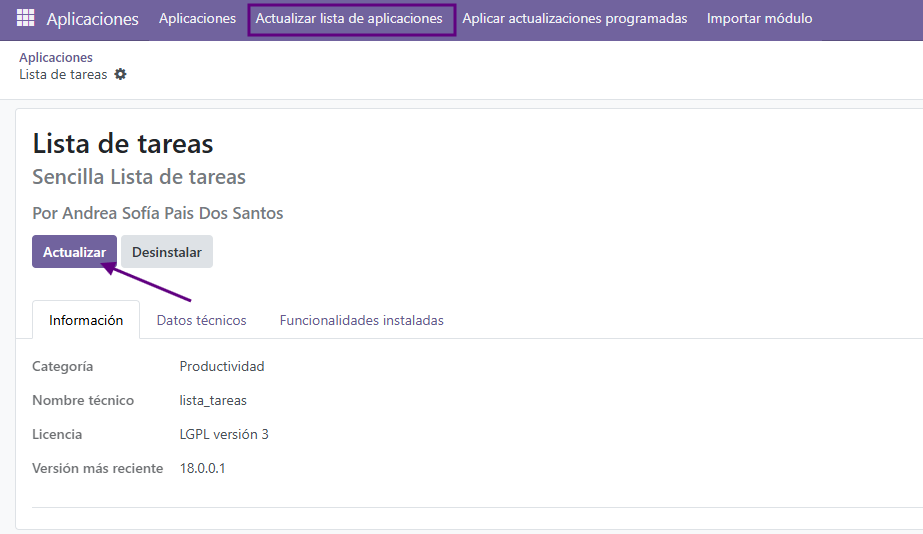
\includegraphics[height=8cm]{images/captura15.png}
\end{center}

Tras actualizar, nos encontramos con algunos cambios al crear una nueva tarea, nos aparece un desplegable con las opciones de categoría que creamos, y nos separa los bloques con un título descriptivo.

\begin{center}
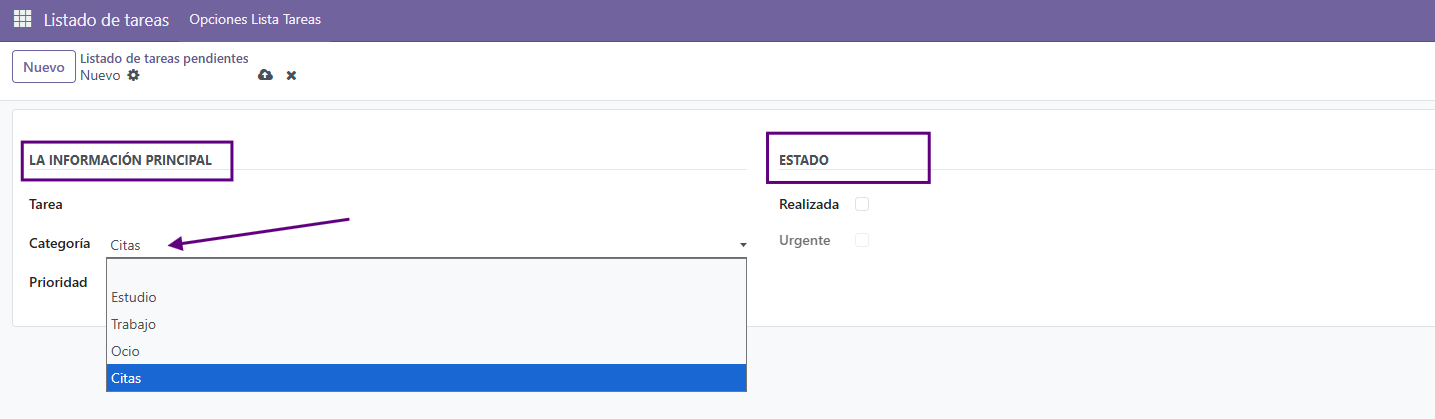
\includegraphics[height=5cm]{images/captura16.png}
\end{center}


\vspace{7cm}
\section{Conclusiones}
En esta práctica pude entender mejor cómo funciona Odoo por dentro y cómo se crean los módulos desde cero. Empecé con algo simple como el módulo “Hola Mundo” y luego pasé al de “Lista de tareas”, donde ya pude aplicar más cosas y ver cómo se conectan los modelos, vistas y datos. 

También me encontré con algunos errores que me ayudaron a entender mejor cómo se estructura todo y cómo solucionarlos. En general, fue una práctica útil para conocer mejor el entorno de desarrollo de Odoo y tener una base para seguir creando módulos más completos más adelante.

\end{document}